%%%%%%%%%%%%%%%%%%%%%%%%%%%%%%%%%%%%%%%%%%%%%%%%%%%%%%%%%%%%%%%%%%%%%%%%%%%%%%%%
% MAE 263F Midterm Progress Report: DiSMech Newton
%%%%%%%%%%%%%%%%%%%%%%%%%%%%%%%%%%%%%%%%%%%%%%%%%%%%%%%%%%%%%%%%%%%%%%%%%%%%%%%%

\documentclass[letterpaper, 10 pt, conference]{ieeeconf}

\IEEEoverridecommandlockouts
\overrideIEEEmargins

\makeatletter
\let\NAT@parse\undefined
\makeatother
\usepackage[numbers]{natbib}
\usepackage{graphicx}
\usepackage{amsmath,amssymb}
\usepackage{booktabs}
\usepackage{placeins}
\usepackage{tikz}
\usetikzlibrary{patterns,arrows.meta,calc,shapes.misc}
\usepackage{algorithm}
\usepackage{algpseudocode}

\newcommand{\solver}{DiSMech Newton}

\title{\LARGE \bf
MAE 263F Midterm Progress Report: \solver
}

\author{Ryan Chaiyakul$^{1}$ and Khai Truong$^{1}$%
\thanks{$^{1}$Department of Mechanical and Aerospace Engineering,
        University of California, Los Angeles, CA 90095, USA.
        {\tt\small ryanchaiyakul@ucla.edu}}%
}

\begin{document}

\maketitle
\thispagestyle{empty}
\pagestyle{empty}

%%%%%%%%%%%%%%%%%%%%%%%%%%%%%%%%%%%%%%%%%%%%%%%%%%%%%%%%%%%%%%%%%%%%%%%%%%%%%%%%
\begin{abstract}
We report midterm progress on \solver, a GPU-native discrete differential geometry (DDG) solver for rods and thin shells in the Newton physics ecosystem.
Since the proposal, we have unified the solver around projected strain-space Gauss--Newton with energy-based contact and Coulomb friction.
We verify the implementation against analytical beam, plate, elastica, overhand knot, and plectoneme theories, and benchmark it against Newton's Vertex Block Descent (VBD) solver.
\end{abstract}

%%%%%%%%%%%%%%%%%%%%%%%%%%%%%%%%%%%%%%%%%%%%%%%%%%%%%%%%%%%%%%%%%%%%%%%%%%%%%%%%
\section{Summary of Proposal and Progress}

Our project develops \solver, a DDG-based solver for slender rods and thin shells inside NVIDIA Newton~\cite{nvidia2025newton}, addressing the unphysical softening and slow force propagation of local-relaxation GPU solvers such as XPBD~\cite{macklin2016xpbd} and VBD~\cite{chen2024vertex}.
The proposal outlined three phases: (1) validation against analytical theory and experimental laws, (2) benchmarks on Newton's cable and cloth examples, and (3) fluid--structure coupling.

\textbf{Changes and Progress Since the Proposal.}
\begin{itemize}
    \item \emph{Projected strain-space Gauss--Newton:} Replaced the initial ADMM prototype~\cite{daviet2023admm} with a unified projected strain-space Gauss--Newton solver (\texttt{SolverDiSMech}) for both rods and midedge shells, using sparse direct linear solves (cuDSS on GPU, SciPy on CPU).
    \item \emph{Energy-based contact and friction:} Implemented barrier-based Offset Geometric Contact (OGC) and Coulomb friction for self-contact, rod--shell contact, and rigid-shape contact within the same step objective.
    \item \emph{Validation and benchmarks:} Completed Phase~1 analytical verifications (rod/shell cantilevers, overhand knot, plectoneme, and heavy-elastica shell fold) and ported Newton's cable and cloth examples (Phase~2). For Phase~3, we have demonstrated viscous fluid drag on helical flagella via external nodal forces; two-way SPH coupling remains for the final report.
\end{itemize}

%%%%%%%%%%%%%%%%%%%%%%%%%%%%%%%%%%%%%%%%%%%%%%%%%%%%%%%%%%%%%%%%%%%%%%%%%%%%%%%%
\section{Physical System Model}

We model rods with Discrete Elastic Rods (DER)~\cite{bergou2008der,bergou2010dvt} and thin shells with midedge Discrete Shells~\cite{grinspun2003des,chen2018midedge}, following DiSMech~\cite{choi2024dismech} (Fig.~\ref{fig:model}).

\begin{figure}[t]
    \centering
    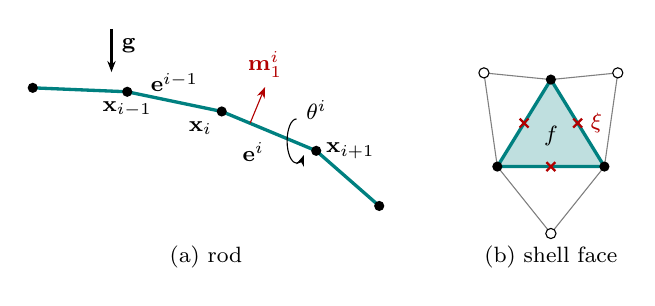
\begin{tikzpicture}[
        node/.style={circle, fill=black, inner sep=1.3pt},
        lbl/.style={font=\footnotesize},
        >={Stealth[length=4pt]}]
        % (a) rod
        \coordinate (x0) at (0,0);
        \coordinate (x1) at (1.2,-0.05);
        \coordinate (x2) at (2.4,-0.3);
        \coordinate (x3) at (3.6,-0.8);
        \coordinate (x4) at (4.4,-1.5);
        \draw[very thick, teal] (x0) -- (x1) -- (x2) -- (x3) -- (x4);
        \foreach \p in {x0,x1,x2,x3,x4} \node[node] at (\p) {};
        \node[lbl, below] at (x1) {$\mathbf{x}_{i-1}$};
        \node[lbl, below left] at (x2) {$\mathbf{x}_{i}$};
        \node[lbl, right] at (x3) {$\mathbf{x}_{i+1}$};
        \node[lbl, above] at ($(x1)!0.5!(x2)$) {$\mathbf{e}^{i-1}$};
        \node[lbl, below left] at ($(x2)!0.55!(x3)$) {$\mathbf{e}^{i}$};
        \coordinate (m) at ($(x2)!0.3!(x3)$);
        \draw[->, red!70!black] (m) -- ++(0.19,0.46) node[lbl, above] {$\mathbf{m}_1^i$};
        \draw[->] ($(x2)!0.75!(x3)+(0.05,0.28)$) arc[start angle=90, end angle=320, x radius=0.12, y radius=0.28];
        \node[lbl, above right] at ($(x2)!0.75!(x3)+(0.05,0.15)$) {$\theta^i$};
        \draw[->, thick] (1.0,0.75) -- (1.0,0.2) node[lbl, right, pos=0.4] {$\mathbf{g}$};
        \node[lbl] at (2.2,-2.15) {(a) rod};
        % (b) shell face
        \begin{scope}[xshift=5.9cm, yshift=-1.0cm, scale=0.85]
            \coordinate (a) at (0,0); \coordinate (b) at (1.6,0); \coordinate (c) at (0.8,1.3);
            \coordinate (fa) at (1.8,1.4); \coordinate (fb) at (-0.2,1.4); \coordinate (fc) at (0.8,-1.0);
            \draw[gray] (b) -- (fa) -- (c) -- (fb) -- (a) -- (fc) -- (b);
            \fill[teal!25] (a) -- (b) -- (c) -- cycle;
            \draw[very thick, teal] (a) -- (b) -- (c) -- cycle;
            \foreach \p in {a,b,c} \node[node] at (\p) {};
            \foreach \p in {fa,fb,fc} \node[circle, draw, fill=white, inner sep=1.3pt] at (\p) {};
            \foreach \u/\v in {b/c, c/a, a/b} \node[cross out, draw, red!70!black, inner sep=1.2pt, thick] at ($(\u)!0.5!(\v)$) {};
            \node[lbl, red!70!black, right] at ($(b)!0.5!(c)+(0.05,0)$) {$\xi$};
            \node[lbl] at (0.8,0.45) {$f$};
        \end{scope}
        \node[lbl] at (6.58,-2.15) {(b) shell face};
    \end{tikzpicture}
    \caption{Degrees of freedom. (a) Discrete elastic rod: nodal positions $\mathbf{x}_i$ and edge twist angles $\theta^i$ about the material frame $\mathbf{m}_1^i$. (b) Midedge shell face $f$: triangle vertices, flap vertices across edges (open), and one midedge angle $\xi$ per edge.}
    \label{fig:model}
\end{figure}

\textbf{Degrees of freedom.}
A rod with $N$ nodes has $4N-1$ DOFs $\mathbf{q} = [\mathbf{x}_0, \theta^0, \mathbf{x}_1, \dots, \mathbf{x}_{N-1}]$.
A triangulated shell has 3 positional DOFs per vertex and 1 midedge bending angle $\xi_e$ per edge.
All bodies share a single global DOF vector $\mathbf{q}$ with lumped mass matrix $\mathbf{M}$.

\textbf{Energies.}
The elastic energy sums quadratic penalties over discrete strains $\boldsymbol{\epsilon}_e(\mathbf{q})$ about their rest values $\bar{\boldsymbol{\epsilon}}_e$ (stretching, bending, and twisting for rod elements; membrane first fundamental form and bending second fundamental form for shell faces):
\begin{equation}
    E_\text{el}(\mathbf{q}) = \sum_{e} \tfrac{1}{2}\big(\boldsymbol{\epsilon}_e(\mathbf{q}) - \bar{\boldsymbol{\epsilon}}_e\big)^{\!\top} \mathbf{K}_e \big(\boldsymbol{\epsilon}_e(\mathbf{q}) - \bar{\boldsymbol{\epsilon}}_e\big).
\end{equation}

\textbf{Forces, contact, and boundary conditions.}
External nodal forces $\mathbf{F}$ include gravity and fluid/air drag.
Self-contact, rod--shell contact, and rigid-shape contact enter as barrier energies $E_\text{c}(\mathbf{q})$ on segment--segment, vertex--triangle, and edge--edge gaps $d$, paired with energy-based Coulomb friction.
Clamped boundaries prescribe fixed DOFs directly to target positions or twist angles.

%%%%%%%%%%%%%%%%%%%%%%%%%%%%%%%%%%%%%%%%%%%%%%%%%%%%%%%%%%%%%%%%%%%%%%%%%%%%%%%%
\section{Algorithm}

Each time step of size $h$ solves implicit Euler by minimizing $\Phi(\mathbf{q})$:
\begin{equation}
    \mathbf{q}_{n+1} = \arg\min_{\mathbf{q}} \tfrac{1}{2h^2}\|\mathbf{q} - \tilde{\mathbf{q}}\|^2_\mathbf{M} + E_\text{el}(\mathbf{q}) + E_\text{c}(\mathbf{q}) - \mathbf{F}^\top\mathbf{q},
    \label{eq:ip}
\end{equation}
with prediction $\tilde{\mathbf{q}} = \mathbf{q}_n + h\mathbf{v}_n$.
Rather than local per-vertex updates as in VBD~\cite{chen2024vertex}, \texttt{SolverDiSMech} uses projected strain-space Gauss--Newton: it assembles a global sparse SPD matrix $\mathbf{A}$ from strain Jacobians $\mathbf{J}_e^\top \mathbf{K}_e \mathbf{J}_e$, geometric stiffness, and contact Hessians, and solves the global system directly via cuDSS on GPU or SciPy on CPU (Algorithm~\ref{alg:step}).

\begin{algorithm}[t]
    \caption{\texttt{SolverDiSMech} time step}
    \label{alg:step}
    \begin{algorithmic}[1]
        \Require $\mathbf{q}_n$, $\mathbf{v}_n$, step $h$, max iterations $K$
        \State $\tilde{\mathbf{q}} \gets \mathbf{q}_n + h \mathbf{v}_n$; $\mathbf{q} \gets \tilde{\mathbf{q}}$ \Comment{predict}
        \State Cap $\mathbf{q} - \mathbf{q}_n$ to contact margin; fallback to $\mathbf{q}_n$ if barrier infinite
        \State Detect contact pairs; assemble and factor $\mathbf{A}$ at $\mathbf{q}$
        \For{$k = 1, \dots, K$}
            \State Evaluate force-balance residual $\mathbf{b} = \nabla \Phi(\mathbf{q})$
            \If{$\|\mathbf{b}\|$ within tolerance} \textbf{break} \EndIf
            \If{exact or contact touching}
                \State Re-assemble and re-factor $\mathbf{A}$ at $\mathbf{q}$
            \EndIf
            \State $\Delta\mathbf{q} \gets -\mathbf{A}^{-1}\mathbf{b}$ \Comment{cuDSS / SciPy}
            \State $\alpha \gets$ backtracking line search, capped at first impact
            \State $\mathbf{q} \gets \mathbf{q} + \alpha\Delta\mathbf{q}$; update material frames \& friction
        \EndFor
        \State $\mathbf{q}_{n+1} \gets \mathbf{q}$; $\mathbf{v}_{n+1} \gets (\mathbf{q}_{n+1} - \mathbf{q}_n)/h$
    \end{algorithmic}
\end{algorithm}

%%%%%%%%%%%%%%%%%%%%%%%%%%%%%%%%%%%%%%%%%%%%%%%%%%%%%%%%%%%%%%%%%%%%%%%%%%%%%%%%
\section{Preliminary Results and Verification}

\subsection{Cantilever Beams and Plates vs. Theory and VBD}

\begin{figure*}[t]
    \centering
    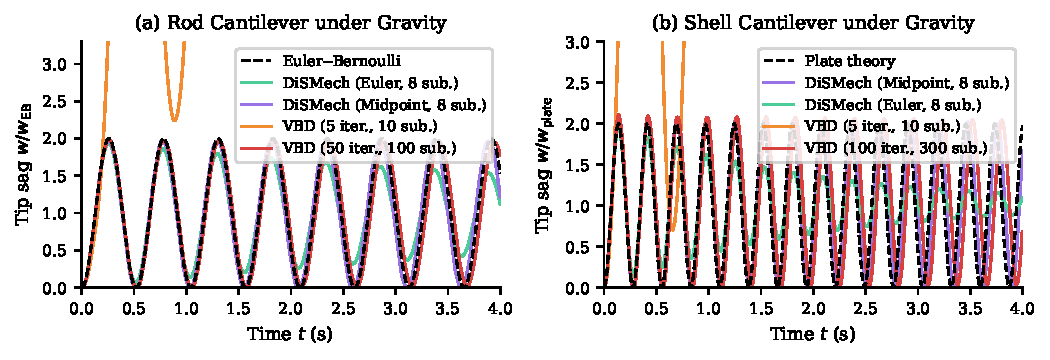
\includegraphics[width=0.96\textwidth]{fig_cantilever.pdf}
    \caption{Cantilever verification under gravity without physical damping. (a) 1.0\,m rod (40 segments, $dt = 1/480$\,s for DiSMech): DiSMech matches Euler--Bernoulli sag ($0.985\,w_\mathrm{EB}$), whereas VBD at 5 iterations softens to $7.99\,w_\mathrm{EB}$ and requires 50 iterations at $dt=1/6000$\,s to match. (b) $0.4\times 0.2$\,m equilateral shell strip: DiSMech (3 iterations, $dt=1/480$\,s) matches Kirchhoff plate theory ($1.009\,w_\mathrm{plate}$), whereas VBD at 5 iterations sags $9.43\,w_\mathrm{plate}$ and requires 100 iterations at $dt=1/18000$\,s.}
    \label{fig:cantilever}
\end{figure*}

Figure~\ref{fig:cantilever} compares \solver{} against analytical theory and Newton's VBD solver on undamped cantilevers under gravity ($g = 9.81\text{ m/s}^2$).
For the 1.0\,m rod (Fig.~\ref{fig:cantilever}a), \solver{} at $dt = 1/480$\,s achieves mean tip sag $0.985\,w_\mathrm{EB}$ and frequency $1.010\,f_\mathrm{EB}$, with implicit midpoint preserving oscillation amplitude ($1.001$ after 1 period) and implicit Euler showing expected numerical damping ($0.927$).
In contrast, VBD with 5 iterations ($dt=1/600$\,s) softens severely to $7.992\,w_\mathrm{EB}$ and requires 50 iterations at $dt = 1/6000$\,s ($12.5\times$ smaller step) to reach $0.988\,w_\mathrm{EB}$.

For the $0.4 \times 0.2\text{ m}$ equilateral shell strip (Fig.~\ref{fig:cantilever}b, $a = 1.15\text{ cm}$), \solver{} needs only 3 iterations at $dt = 1/480$\,s to match Kirchhoff plate theory ($1.009\,w_\mathrm{plate}$ sag, $0.998\,f_\mathrm{plate}$ frequency).
Because VBD propagates corrections one vertex ring per iteration across a membrane $10^5\times$ stiffer than bending, VBD at 5 iterations sags $9.431\,w_\mathrm{plate}$ at $0.448\,f_\mathrm{plate}$, requiring 100 iterations at $dt = 1/18000$\,s ($37.5\times$ smaller step) to reach $1.047\,w_\mathrm{plate}$.
Mesh refinement of the midedge shell at triangle side lengths $2.3$, $1.15$, and $0.58\text{ cm}$ converges monotonically to plate theory with sag errors of $2.3\%$, $1.4\%$, and $0.5\%$, respectively.

\subsection{Self-Contact, Friction, and Heavy Elastica}

\begin{figure*}[t]
    \centering
    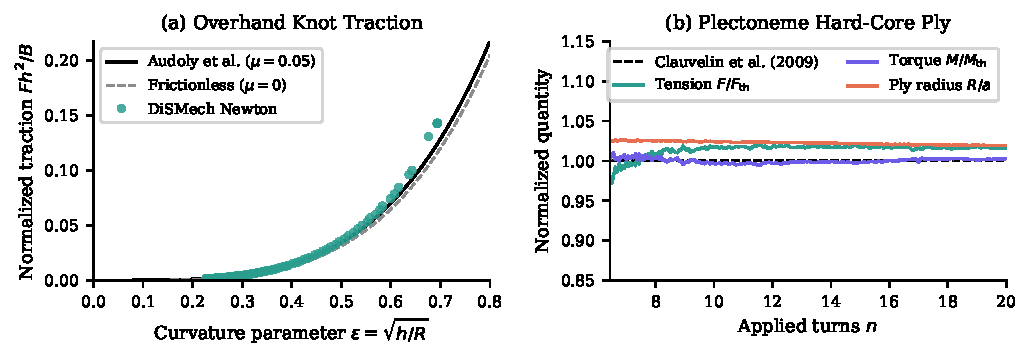
\includegraphics[width=0.96\textwidth]{fig_theory_contact.pdf}
    \caption{Self-contact and friction verification. (a) Overhand knot ($\mu = 0.05$) pulled tight: normalized traction $F h^2 / B$ versus curvature parameter $\varepsilon = \sqrt{h/R}$ matches Audoly et al.~\cite{audoly2007knots} (median ratio $0.999$, $N=629$ sliding frames) with minimum gap $0.995\,D$. (b) Twisted rod plectoneme ($n$ turns): normalized tension $F/F_\mathrm{th}$, torque $M/M_\mathrm{th}$, and ply radius $R/a$ closely track Clauvelin et al.~\cite{clauvelin2009plectoneme}.}
    \label{fig:theory_contact}
\end{figure*}

Figure~\ref{fig:theory_contact} validates energy-based self-contact and Coulomb friction against analytical theories:
\begin{itemize}
    \item \emph{Overhand knot} (Fig.~\ref{fig:theory_contact}a): Pulling a loose trefoil knot ($\mu = 0.05$) yields a median normalized traction $F h^2 / B$ ratio of $0.999$ relative to Audoly et al.~\cite{audoly2007knots} ($F h^2 / B = \tfrac{1}{2}\varepsilon^4 + \mu\sigma\varepsilon^3$, $\sigma=0.492$) over 629 sliding frames, with zero interpenetration (minimum gap $0.995\,D$).
    \item \emph{Plectoneme} (Fig.~\ref{fig:theory_contact}b): Twisting a 0.5\,m slack rod by 20 turns (500 segments, frictionless) forms a hard-core ply matching Clauvelin et al.~\cite{clauvelin2009plectoneme} across 218 ply frames: median tension $F/F_\mathrm{th} = 1.017$ (range $0.971\text{--}1.021$), median torque $M/M_\mathrm{th} = 0.999$ ($0.994\text{--}1.010$), median ply radius $R/a = 1.023$ ($1.019\text{--}1.027$), and exact linking-number conservation ($\max |\mathrm{Lk} - n| < 10^{-4}$).
    \item \emph{Shell fold}: Dropping a $0.8 \times 0.15\text{ m}$ cloth strip onto itself settles into an eyelet within $\sim 1\%$ of the frictionless heavy elastica height $0.907\,(D / \rho g)^{1/3}$.
\end{itemize}

\begin{table}[!h]
    \centering
    \caption{Summary of Analytical and Convergence Verification}
    \label{tab:verification}
    \setlength{\tabcolsep}{4pt}
    \resizebox{\columnwidth}{!}{%
    \begin{tabular}{@{}lll@{}}
        \toprule
        Benchmark & Target / Reference & Measured Result \\
        \midrule
        Rod cantilever & Euler--Bernoulli & Sag $0.985\,w_\mathrm{EB}$, freq. $1.010\,f_\mathrm{EB}$ \\
        Shell cantilever & Kirchhoff plate & Sag $1.009\,w_\mathrm{plate}$, freq. $0.998\,f_\mathrm{plate}$ \\
        Shell mesh conv. & $a = 2.3, 1.15, 0.58$\,cm & Error $2.3\%, 1.4\%, 0.5\%$ \\
        Overhand knot & Audoly et al.~\cite{audoly2007knots} & Median ratio $0.999$, gap $0.995\,D$ \\
        Plectoneme & Clauvelin et al.~\cite{clauvelin2009plectoneme} & $F/F_\mathrm{th}=1.017$, $M/M_\mathrm{th}=0.999$ \\
        Shell fold & Heavy elastica & Within $\sim 1\%$ of $0.907(D/\rho g)^{1/3}$ \\
        \bottomrule
    \end{tabular}}
\end{table}

Table~\ref{tab:verification} summarizes our quantitative verification across all analytical benchmarks.
In addition, Newton's canonical cable and cloth examples (cable twist, pile, plectoneme, Y-junction, hanging cloth, cloth bending, and cloth twist) all run end-to-end on \texttt{SolverDiSMech}.

\FloatBarrier
%%%%%%%%%%%%%%%%%%%%%%%%%%%%%%%%%%%%%%%%%%%%%%%%%%%%%%%%%%%%%%%%%%%%%%%%%%%%%%%%
\bibliographystyle{IEEEtran}
\bibliography{midterm}

\end{document}
